

\chapter{测试框架设计}

在本部分中,将对整个测试框架的结构进行设计并描述该设计相对于已有的一些测试框架所具有的优势。

\section{总体设计}
对于整个测试框架,我们将其分为下面的几个部分:
\begin{itemize}
\item 内核编译系统。用于进行内核的编译工作,能够自动化的内核代码管理,以及内核编译任务管理,处理各种与编译相关的任务。
\item 测试管理系统。测试管理系统管理整个测试的流程以及进行测试任务的分配和测试机器的协调。
\end{itemize}

图\ref{fig:compile_test_relation}中表现了内核编译系统和测试管理系统之间的关系。测试管理系统会根据需要向内核编译系统提交内核编译任务,内核编译系统会将编译完成的内核提供给测试管理系统进行性能测试。

\begin{figure}[H]
\centering
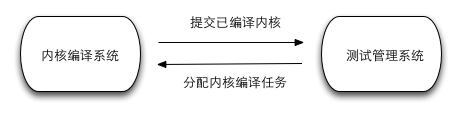
\includegraphics[width=12cm]{compile_test_relation}
\caption{内核编译系统与测试管理系统}
\label{fig:compile_test_relation}
\end{figure}

下面我们也将按照这两个系统对框架的设计进行介绍。

\subsection{内核编译系统}
内核的编译是一个非常耗时的过程,要想进行高效率的性能测试工作,那么高效率的内核编译是必不可少的。

图\ref{fig:compile_manage}中介绍的是内核编译系统的大致结构,整个内核编译系统可以分为两个部分:

\begin{itemize}
\item 编译管理服务器

编译管理服务器是整个内核编译系统的核心,编译管理服务器具有一下的职责:

\begin{enumerate}
\item 更新并合并各分支的内核源代码
\item 从测试管理系统获取编译任务
\item 将编译任务分配给每一个编译节点
\item 从编译节点获取编译完成的内核镜像
\item 向测试管理系统提供编译完成的内核
\end{enumerate}

\item 编译节点

每一个编译节点都是一台真实的计算机,并且运行的流程非常简单:
\begin{enumerate}
\item 
\item
\item
\item
\end{enumerate}

\end{itemize}

\begin{figure}[H]
\centering
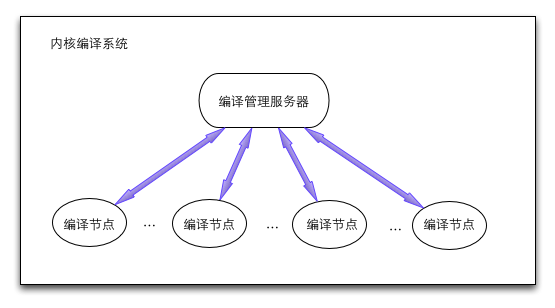
\includegraphics[width=12cm]{compile_manage}
\caption{内核编译系统结构}
\label{fig:compile_manage}
\end{figure}

\subsection{测试管理系统}
\subsubsection{性能测试配置}
要进行性能测试,自然是需要有能够用于运行待测试内核的测试机,为了能够尽可能地提高性能测试效率,在我们的测试框架中,我们将使用具有Linux内核支持的KVM虚拟机来进行相关的测试工作。

在一台真实的计算机上,可以同时运行多台使用KVM技术的虚拟机,更为方便的是KVM虚拟机支持使用指定的内核和内存镜像文件来运行,这样,我们就可以不用花费大量的时间来进行内核镜像和内存镜像文件的打包,因此,使用虚拟机来进行内核的性能测试能够大大提高测试的效率。

另外,使用虚拟机还可以简化硬件的配置,因为虚拟机的硬件配置都是可以进行配置的,这样,可以使得我们的内核能够在更多的复杂硬件环境中运行,就更有可能发现内内核中存在的性能回退问题。

随着近几年来虚拟机技术的发展,越来越多的主机运营商也开始使用虚拟机来提供主机业务,因此虚拟机上的I/O性能也逐渐受到重视,因此使用虚拟机来进行内核性能测试是非常有必要的。

当然,我们的测试框架中所使用的不仅仅是虚拟机,毕竟虚拟机中的硬件模拟和真实硬件之间还是存在着比较大的区别,虚拟机测试是不能完全替代真机测试的,我们的测试是能够在真机上轻松运行。



\subsubsection{测试运行流程}

在多个测试服务器之间相互通信。

\subsubsection{问题自动定位}
在我们的测试框架中,我们将会对某个版本的内核进行测试,并使用一定的算法来处理这些测试数据,从中找到性能回退问题。

一旦找到性能回退的问题,我们会再次进行测试以确认这个回退问题,在确认性能回退问题之后,我们将会开始对造成这个性能回退问题的代码进行定位。

一般来说,性能回退问题往往是由某一次或者多次的修改造成的,我们的目标就是定位到造成性能回退问题的这一次修改。



\section{提升与优势}

我们新设计的框架相对于已有的一些测试框架和具有相似功能的框架相比具有很大的提升和更多的优势。

\begin{itemize}
\item 与LKP相比

\begin{enumerate}
\item 覆盖更多的开发分支,能够更早地发现潜在的性能回退
\item 具有更高的测试效率
\item 拥有更加全面和完善的数据处理和分析能力
\item 提供更加详细,更加丰富的测试结果报告
\item 尽可能充分利用已有的计算资源
\end{enumerate}

\item 与MMTests相比

\begin{enumerate}
\item 拥有更为完善和统一的数据处理流程
\item 拥有更全面的测试数据覆盖
\item 具有更完整的测试流程
\item 具有数据分析功能
\item 具有问题定位功能
\end{enumerate}

\end{itemize}